\section{Prospetto economico}
In questa sezione è presentato il prospetto economico del progetto, suddiviso per fasi. Il costo è calcolato utilizzando i dati
della tabella al paragrafo 5.

%-----------------------------------------------------------------------------------------------------
%-------------------------------------- ANALISI ------------------------------------------------------
%-----------------------------------------------------------------------------------------------------
\subsection{Analisi}
A scopo di trasparenza viene redatto il prospetto economico riguardante la fase di Analisi dei Requisiti, che si precisa essere a carico del fornitore, e non del proponente.

\begin{table}[H]
	\centering
	\begin{tabular}{ l c c }
		\textbf{Ruolo} & \textbf{Ore} & \textbf{Costo} \\
		\hline
		Amministratore & 30 & 600 ? \\
		Analista & 58 & 1450 ? \\
		Progettista & 9 & 198 ? \\
		Programmatore & 0 & 0 ? \\
		Responsabile & 14 & 420 ? \\
		Verificatore & 31 & 465 ? \\
		\hline
		Totale & 142 & 3133 ? \\
		\hline
	\end{tabular}
	\caption{Ore e costo per ruolo, periodo di Analisi}
\end{table}

I seguenti grafici mostrano il peso orario e di costo di ogni ruolo in questo periodo.

\begin{figure}[H]
  \begin{center}
    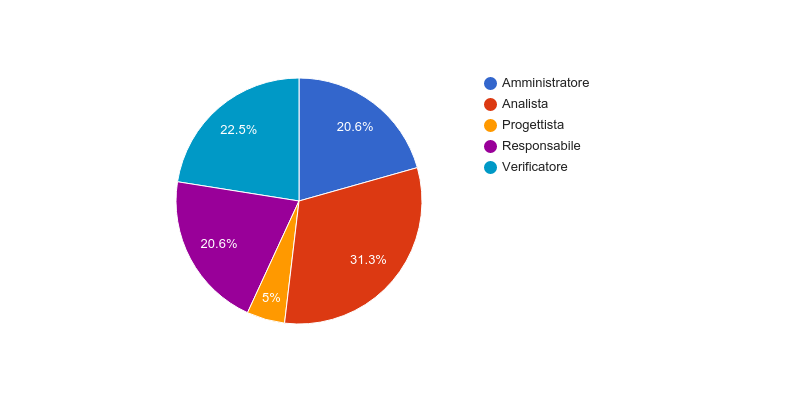
\includegraphics[width=12cm]{res/img/orePerRuoloAnalisi.png}
  \caption{Ore per componente, fase di Analisi}
  \end{center} 
\end{figure}  

\begin{figure}[H]
  \begin{center}
    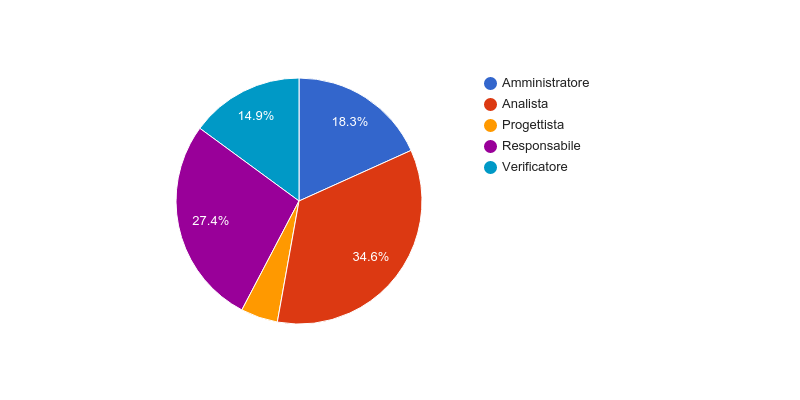
\includegraphics[width=12cm]{res/img/costoPerRuoloAnalisi.png}
  \caption{Costo per ruolo, fase di Analisi}
  \end{center} 
\end{figure}  


%-----------------------------------------------------------------------------------------------------
%-------------------------------------- PROGETTAZIONE ARCHITETTURALE ---------------------------------
%-----------------------------------------------------------------------------------------------------
\subsection{Progettazione Architetturale}
Nella fase di Progettazione Architetturale le ore per ogni ruolo sono state cos\`i suddivise:

\begin{table}[H]
	\centering
	\begin{tabular}{ l c c }
		\textbf{Ruolo} & \textbf{Ore} & \textbf{Costo} \\
		\hline
		Amministratore & 30 & 600 ? \\
		Analista & 58 & 1450 ? \\
		Progettista & 9 & 198 ? \\
		Programmatore & 0 & 0 ? \\
		Responsabile & 14 & 420 ? \\
		Verificatore & 31 & 465 ? \\
		\hline
		Totale & 142 & 3133 ? \\
		\hline
	\end{tabular}
	\caption{Ore e costo per ruolo, periodo di Progettazione Architetturale}
\end{table}

I seguenti grafici mostrano il peso orario e di costo di ogni ruolo in questo periodo.

\begin{figure}[H]
  \begin{center}
    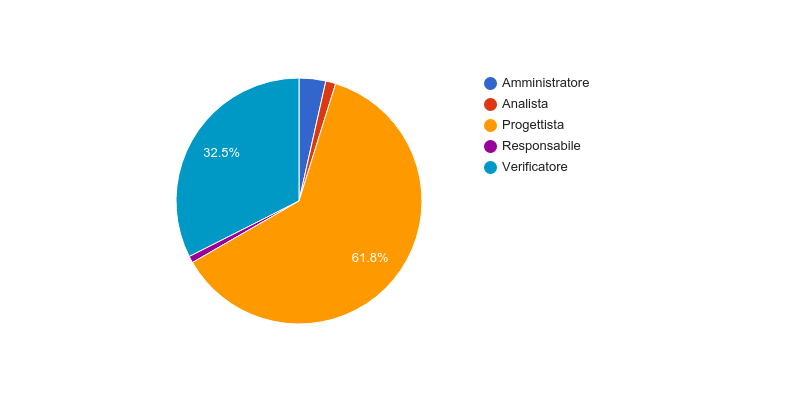
\includegraphics[width=12cm]{res/img/orePerRuoloProgettazioneArchitetturale.png}
  \caption{Ore per componente, fase di Progettazione Architetturale}
  \end{center} 
\end{figure}  

\begin{figure}[H]
  \begin{center}
    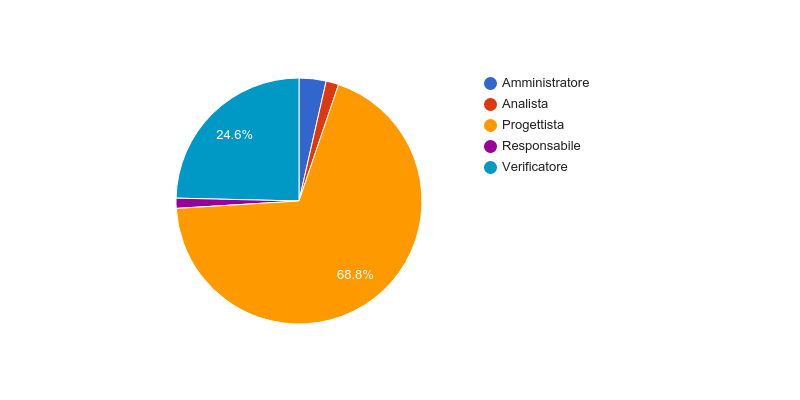
\includegraphics[width=12cm]{res/img/costoPerRuoloProgettazioneArchitetturale.png}
  \caption{Costo per ruolo, fase di Progettazione Architetturale}
  \end{center} 
\end{figure}  


%-----------------------------------------------------------------------------------------------------
%-------------------------------------- PROGETTAZIONE DI DETTAGLIO E CODIFICA ------------------------
%-----------------------------------------------------------------------------------------------------
\subsection{Progettazione di dettaglio e codifica}
Nel periodo di Progettazione di Dettaglio e Codifica le ore per ogni ruolo sono state così suddivise:

\begin{table}[H]
	\centering
	\begin{tabular}{ l c c }
		\textbf{Ruolo} & \textbf{Ore} & \textbf{Costo} \\
		\hline
		Amministratore & 30 & 600 ? \\
		Analista & 58 & 1450 ? \\
		Progettista & 9 & 198 ? \\
		Programmatore & 0 & 0 ? \\
		Responsabile & 14 & 420 ? \\
		Verificatore & 31 & 465 ? \\
		\hline
		Totale & 142 & 3133 ? \\
		\hline
	\end{tabular}
	\caption{Ore e costo per ruolo, periodo di Progettazione di Dettaglio e Codifica}
\end{table}

I seguenti grafici mostrano il peso orario e di costo di ogni ruolo in questo periodo.

\begin{figure}[H]
  \begin{center}
    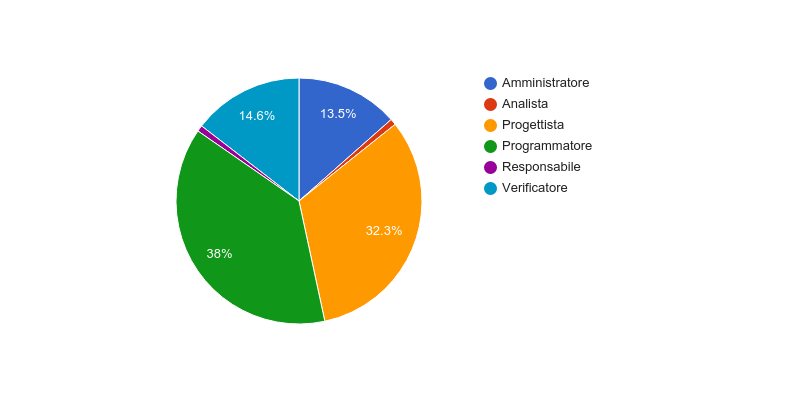
\includegraphics[width=12cm]{res/img/orePerRuoloProgettazioneDettaglioCodifica.png}
  \caption{Ore per componente, fase di Progettazione di Dettaglio e Codifica}
  \end{center} 
\end{figure}  

\begin{figure}[H]
  \begin{center}
    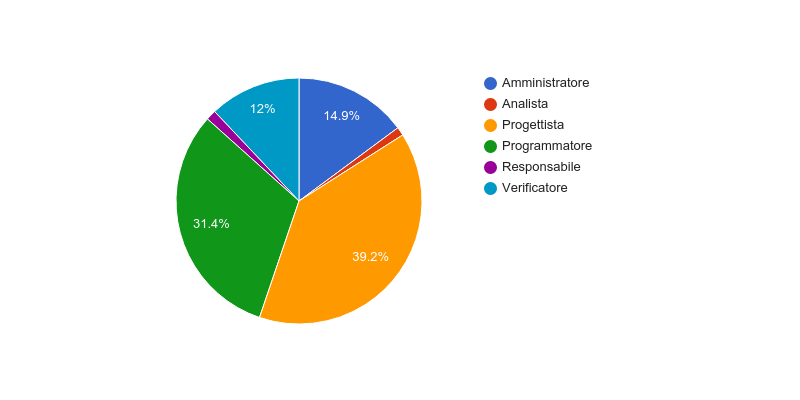
\includegraphics[width=12cm]{res/img/costoPerRuoloProgettazioneDettaglioCodifica.png}
  \caption{Costo per ruolo, fase di Progettazione di Dettaglio e Codifica}
  \end{center} 
\end{figure}  


%-----------------------------------------------------------------------------------------------------
%-------------------------------------- VALIDAZIONE --------------------------------------------------
%-----------------------------------------------------------------------------------------------------
\subsection{Validazione}
Nel periodo di Validazione le ore per ogni ruolo sono state cosi suddivise:

\begin{table}[H]
	\centering
	\begin{tabular}{ l c c }
		\textbf{Ruolo} & \textbf{Ore} & \textbf{Costo} \\
		\hline
		Amministratore & 30 & 600 ? \\
		Analista & 58 & 1450 ? \\
		Progettista & 9 & 198 ? \\
		Programmatore & 0 & 0 ? \\
		Responsabile & 14 & 420 ? \\
		Verificatore & 31 & 465 ? \\
		\hline
		Totale & 142 & 3133 ? \\
		\hline
	\end{tabular}
	\caption{Ore e costo per ruolo, periodo di Validazione}
\end{table}

I seguenti grafici mostrano il peso orario e di costo di ogni ruolo in questo periodo.

\begin{figure}[H]
  \begin{center}
    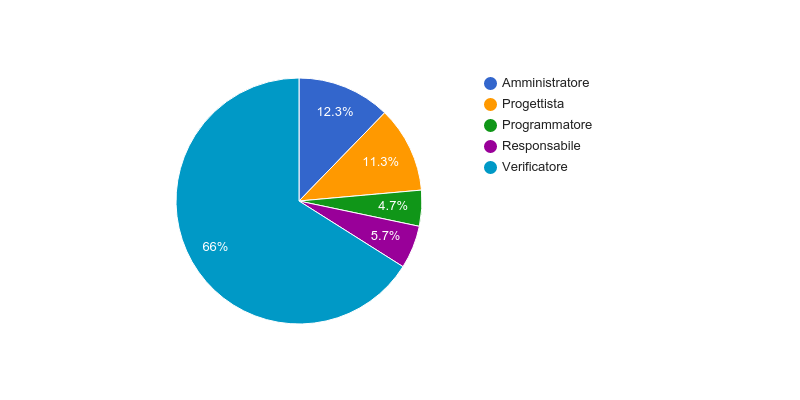
\includegraphics[width=12cm]{res/img/orePerRuoloValidazione.png}
  \caption{Ore per componente, fase di Validazione}
  \end{center} 
\end{figure}  

\begin{figure}[H]
  \begin{center}
    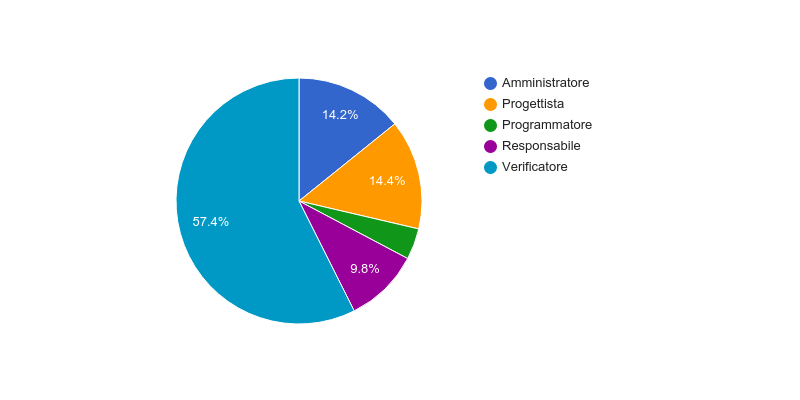
\includegraphics[width=12cm]{res/img/costoPerRuoloValidazione.png}
  \caption{Costo per ruolo, fase di Validazione}
  \end{center} 
\end{figure}  


%-----------------------------------------------------------------------------------------------------
%-------------------------------------- TOTALE -------------------------------------------------------
%-----------------------------------------------------------------------------------------------------
\subsection{Totale}
In totale le ore per ogni ruolo sono state così suddivise:

\begin{table}[H]
	\centering
	\begin{tabular}{ l c c }
		\textbf{Ruolo} & \textbf{Ore} & \textbf{Costo} \\
		\hline
		Amministratore & 30 & 600 ? \\
		Analista & 58 & 1450 ? \\
		Progettista & 9 & 198 ? \\
		Programmatore & 0 & 0 ? \\
		Responsabile & 14 & 420 ? \\
		Verificatore & 31 & 465 ? \\
		\hline
		Totale & 142 & 3133 ? \\
		\hline
	\end{tabular}
	\caption{Ore e costo per ruolo, riassunto progetto}
\end{table}

Il seguente grafico mostra il costo di ogni ruolo durante tutto lo svolgimento del progetto, escluso il periodo di Analisi dei Requisiti.

\begin{figure}[H]
  \begin{center}
    \includegraphics[width=12cm]{res/img/orePerRuoloRiassuntoProgetto.png}
  \caption{Ore per componente, riassunto progetto}
  \end{center} 
\end{figure}  

\begin{figure}[H]
  \begin{center}
    \includegraphics[width=12cm]{res/img/costoPerRuoloRiassuntoProgetto.png}
  \caption{Costo per ruolo, riassunto progetto}
  \end{center} 
\end{figure}  


